\documentclass{article}
\usepackage[utf8]{inputenc}
\usepackage{amsmath}
\usepackage{graphicx,float}
\usepackage{caption}
\usepackage{subcaption}
\usepackage[margin=1.25in]{geometry}

\title{Synthesis}
\author{Alex Booth\\ a.booth9@edu.salford.ac.uk}
\date{October 2022}

\begin{document}

\maketitle
\section{Abstract}
    \textit{Here goes the abstract}
\newpage
\tableofcontents
\newpage

\section{Introduction}
    Musical instruments have been part of human culture and craft since prehistory, playing a part in both written and verbal art, ceremony and celebration \cite{rault}.
    This report describes an attempted recreation using digital synthesis of two acoustic musical instruments from the western European musical tradition: a mandolin and a flute.
    Acoustic musical instruments use an excited string, SOMETHING OR SOMETHING - REF to generate waves which are manipulated and shaped by the body or of the musical instrument NEEDS A TIED-IN CITATION. % CITE
    
    The generation of these waves, and their manipulation by the body of the musical instrument can be modelled using a series of oscillators, filters and modulators.
    Audio synthesis using analog circuitry was explored as soon as simple oscillators were readily available, leading to early electronic musical instruments such as the theremin.  % WHEN? 
    The synthesis of musical instruments can be achieved using many techniques.
    In order to emulate the sound of musical instruments using synthesis, first we must understand the mathematical nature of sound as a signal.
    Thus, this report will describe the programmatic mathematical analysis of the aforementioned two recordings, and an attempt to use the data gathered in the analysis to guide the chosen synthesis technique. 
    

\section{Theory}
    \subsection{Signal processing, generation and analysis}
        Sound can be understood as a signal which is a function of time.
        As sound travels in air it is a longitudinal pressure wave, whilst when in the electronic domain, such as after transduction by a microphone, it is transverse wave of voltage as a function of time CITE?.
        When transformed from the analogue electronic domain to the digital domain, the signal remains a transverse wave and a function of time.
        However, it changes from a continuously changing voltage to a numerical sample value that increments in discreet steps. CITE
        
        Any periodic continuous signal can be broken down into an infinite sum of weighted sine and cosine waves \cite{weisstein2004fourier}.
        A further development of the theoretical foundation began with the Fourier series can be found in the Fourier transform, which in continuous time takes the form:
        \begin{equation}
            X(\omega) = \int_{-\infty}^{+\infty}x(t)e^{-j\omega t}dt
            \label{contFourier}
        \end{equation}
        However, as digital audio works in the discrete time domain, the integral seen in Eq.\ref{contFourier} is changed to a sum and the Fourier transform becomes:
        \begin{equation}
            X(\omega) = \sum_{-\infty}^{+\infty}x[n]e^{-j\omega t}dt
        \end{equation}
        In the 1960s, J.W. Cooley and John Tukey developed an algorithm to efficiently compute the discrete Fourier transform \cite{cooley1965algorithm}.
        This, and other discrete-time Fourier transform algorithms, became known as the fast Fourier transform(s) (FFT).
        MATLAB's in-built FFT function uses an FFT algorithm from the the FFTW library \cite{frigo1998fftw}, which builds on Cooley and Tukey's original FFT.
        Using a Fourier transform, a complex signal of any length such as a musical note or speech excerpt, can be broken down into it's frequency components, showing their respective magnitudes averaged over the length in time of the signal.
        Phase information can be extracted from the Fourier transform, but this information was not particularly useful for the purposes of the synthesis described in this report.
        
        The Fourier transform allows the fundamental frequency and harmonics of the played note to be identified, due to the fact that in a good quality recording they will be the most prominent components of the frequency spectrum.
        However, the Fourier transform does not only show the harmonic or musical frequency content of a signal, instead it shows all the frequency content of a signal.
        As such, any noise or other anharmonic frequency component, musical or not, will be shown on the transform.
        Thus, the simple inclusion of all observed frequency components may or may not be constructive to emulating the original played note.
        For example, this may include unwanted recording artifacts.
        
        Early musical synthesizers were constructed to facilitate additive synthesis techniques.
        This is where a series of oscillators generate basic waveforms such as sines, sawtooth and pulse waves; a sawtooth wave can be seen in Figure \ref{sawtooth}.
        \begin{figure}[H]
            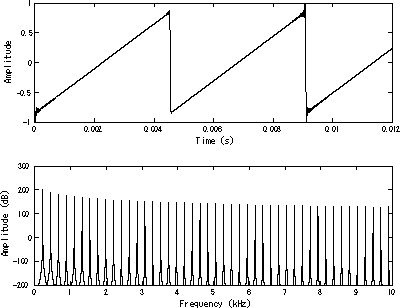
\includegraphics[scale=0.6]{images/Sawtooth.png}%
            \centering
            \caption{Waveform and frequency response of a sawtooth wave.}\cite{kraft2017lp}
            \label{sawtooth}
        \end{figure}
        
        These oscillators may be used to generate sound, or used as modulators to other oscillators's outputs.
        Shown in Fig. \ref{oscBank} is an oscillator bank from a synthesizer, it illustrates the basic wave shapes that were available as building blocks for additive synthesis.
        \begin{figure}[H]
            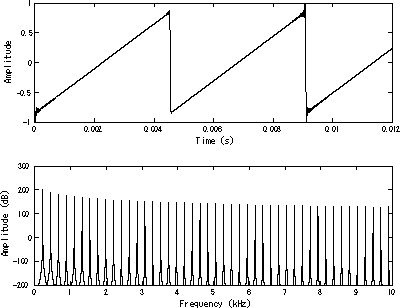
\includegraphics[scale=0.6]{images/Sawtooth.png}%
            \centering
            \caption{Waveform and frequency response of a sawtooth wave.}\cite{kraft2017lp}
            \label{oscBank}
        \end{figure}
        Different waveforms generated by these oscillators will have a different harmonic content.
        For example: in Figure \ref{sawtooth} a sawtooth wave is shown as having many harmonics in it's frequency domain plot.
        In fact, a sawtooth wave contains all harmonics both even and odd, of a fundamental tone \cite{roederer1995physics}.
        
        In the 1970s, FM synthesis was beginning to take form as a method of musical instrument emulation, especially after Chowning's work outlined specific FM techniques for the emulation of various instruments \cite{chowning1973synthesis}.
        Products such as the Yamaha DX7 helped to popularize FM synthesis into the 1980s.
        
    \subsection{Musical instruments}

\section{Methodology}
    \subsection{Analysis}
        \subsubsection{Mandolin}
            All code written for this report was executed in MATLAB.
            First, the sample values and sampling rates of the recordings were imported into MATLAB as a vector and constant, respectively.
            Using the sampling rate and total number of samples, a vector of time data was created.
            This allowed the sample values to be plotted against time, as seen in Figure \ref{timeDomainMando}.
            \begin{figure}[H]
                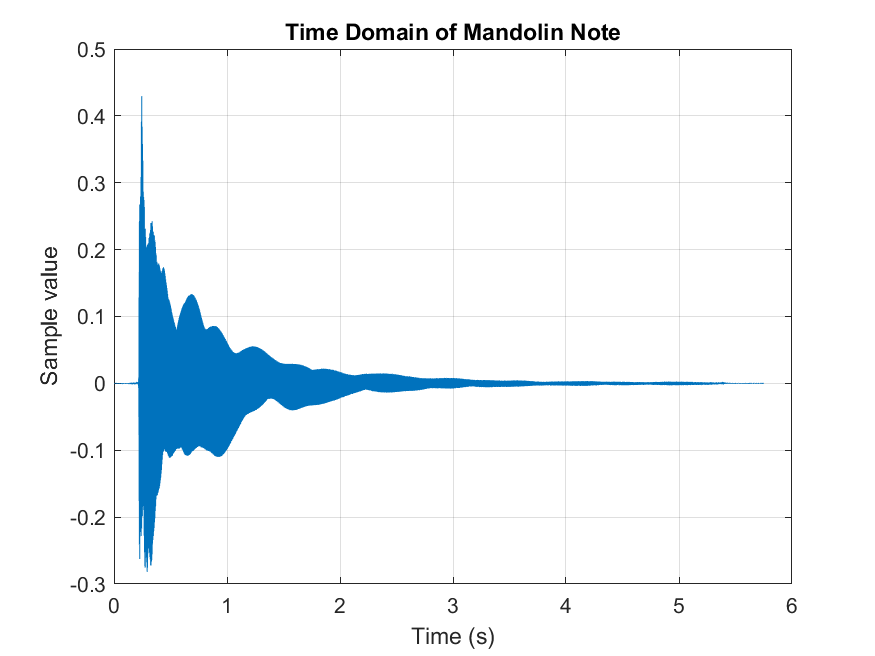
\includegraphics[scale=0.5]{images/timeDomainMando.png}%
                \centering
                \caption{Mandolin sample value over time.}
                \label{timeDomainMando}
            \end{figure}
            
            Next, analysis of the signal in the frequency domain was performed.
            Using MATLAB's in-built FFT function, a frequency domain plot of the signal, averaged over time, was plotted.
            \begin{figure}[H]
                \centering
                \begin{minipage}{.49\textwidth}
                    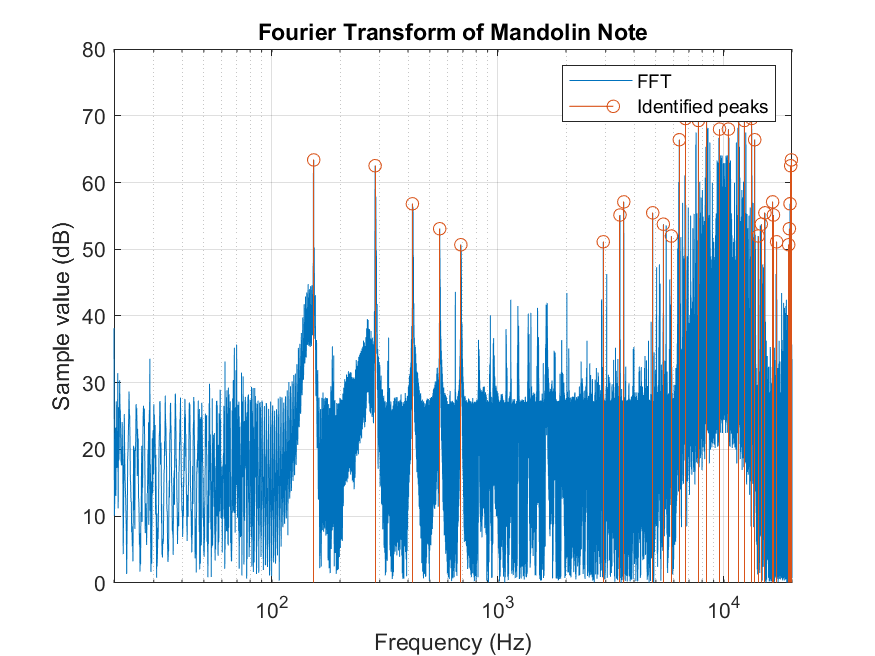
\includegraphics[width=\linewidth]{images/FFTMando.png}%
                    \centering
                    \caption{Mandolin sample value over time.}
                    \label{FFTMando}
                \end{minipage}
                \begin{minipage}{.49\textwidth}
                    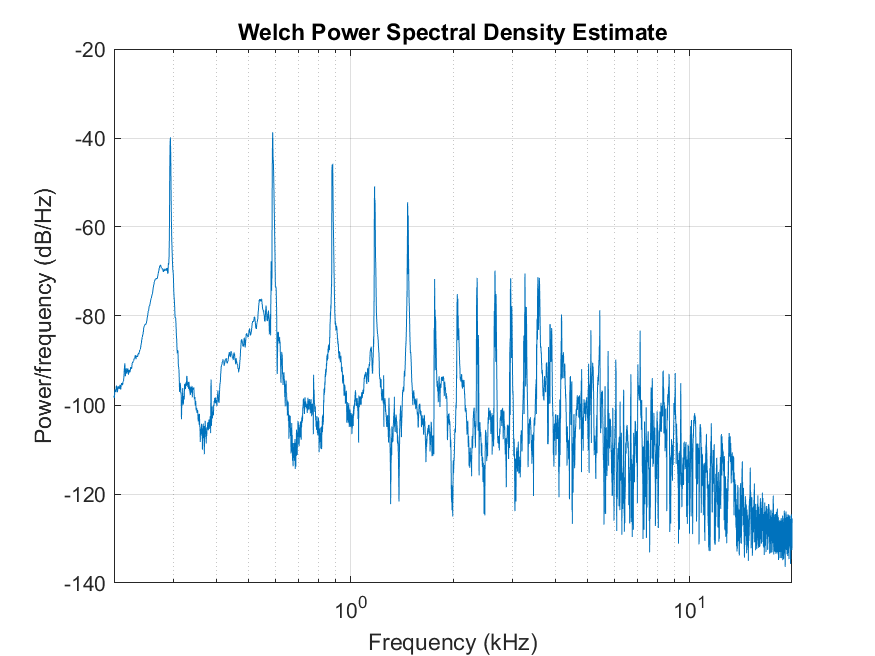
\includegraphics[width=\linewidth]{images/welchMando.png}%
                    \centering
                    \caption{Mandolin sample value over time.}
                    \label{welchMando}
                \end{minipage}
            \end{figure}
            This data was supplemented with another frequency domain plot using \texttt{pwelch()}, a function that uses the Welch algorithm to obtain power spectral density as a function of frequency, instead of sample magnitude \cite{solomon1991psd}.
            A plot of the frequency and phase responses generated by \texttt{pwelch()} are shown in Figure \ref{welchMando}.

            The frequency amplitude information gathered from the Fourier transform and Welch power spectral density estimate is averaged over the entire duration of the signal.
            While this information is very useful, it is limited: Much of the frequency content of a signal varies in time, and this time-varying nature of the frequency response contributes greatly to the 
            To see the amplitudes of each frequency component as a function of time, a spectrogram was used.

            MATLAB's \texttt{spectrogram()} function has a high degree of operability and can take many arguments.
            The function works using a 
            Used as a standalone function, it gives the user a two dimensional graph of frequency versus time, with frequency amplitude as a third, coloured dimension.
            There is a trade-off between resolution in the frequency and time domains when using this spectrogram function.
            Higher resolution in the time domain allows for a more visually understandable spectrogram when using a waterfall plot.
            If a high frequency-domain resolution is used, a waterfall plot becomes cluttered and hard to read, as shown 
            Using a hamming window with length $n = 2560$, a 2650-point spectrogram was computed and plotted on a waterfall graph, shown in Figure \ref{specWaterfallMando1}.
            \begin{figure}[H]
                \centering
                \begin{minipage}{.49\textwidth}
                    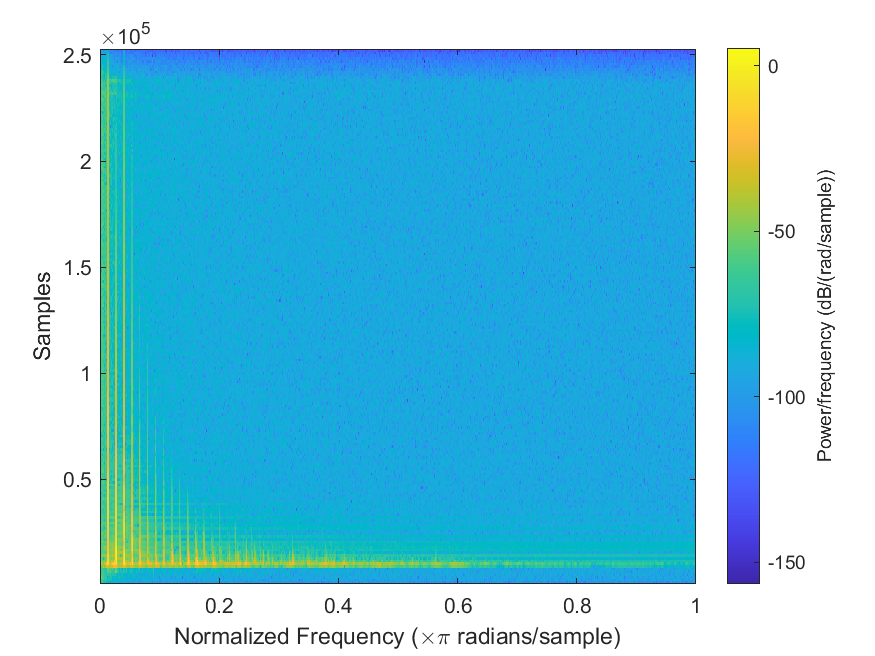
\includegraphics[width=\linewidth]{images/specMando.png}%
                    \centering
                    \caption{Mandolin sample value over time.}
                    \label{specMando1}
                \end{minipage}
                \begin{minipage}{.49\textwidth}
                    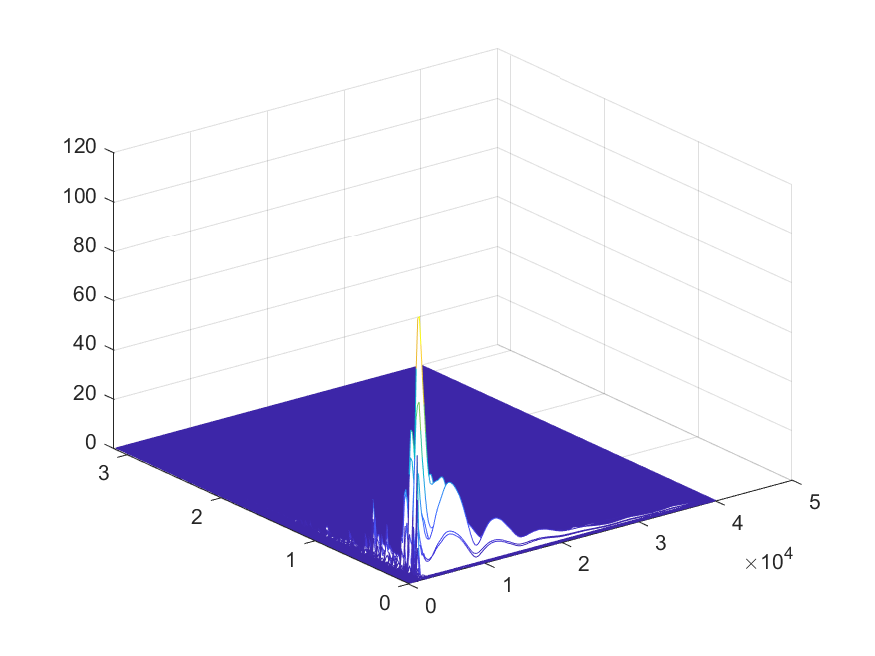
\includegraphics[width=\linewidth]{images/specWaterfallMando1.png}%
                    \centering
                    \caption{Waterfall plot of mandolin frequency-domain amplitudes with respect to time.}
                    \label{specWaterfallMando1}
                \end{minipage}
            \end{figure}
            \newpage
            
        \subsubsection{Flute}
            Much like with the mandolin, time and frequency domain plots were generated of the flute recording.
            These can be seen in Figs.\ref{timeDomainFlute}, \ref{FFTFlute}, \ref{fluteWelch} and \ref{fluteSpec}.
            \begin{figure}[H]
                \centering
                \begin{minipage}{.49\textwidth}
                    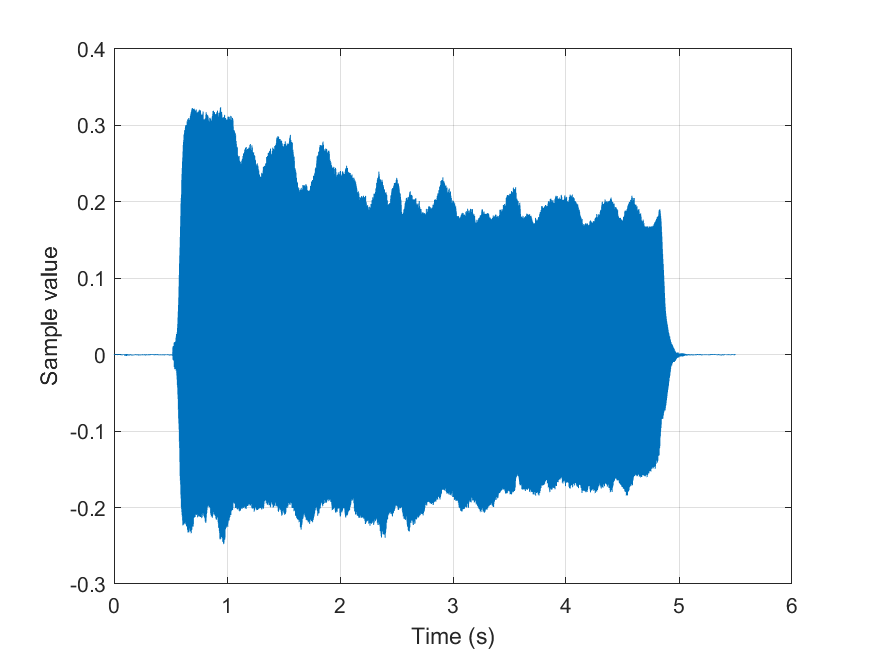
\includegraphics[width=\linewidth]{images/timeDomainFlute.png}%
                    \centering
                    \caption{Time-domain of the flute recording.}
                    \label{timeDomainFlute}
                \end{minipage}
                \begin{minipage}{.49\textwidth}
                    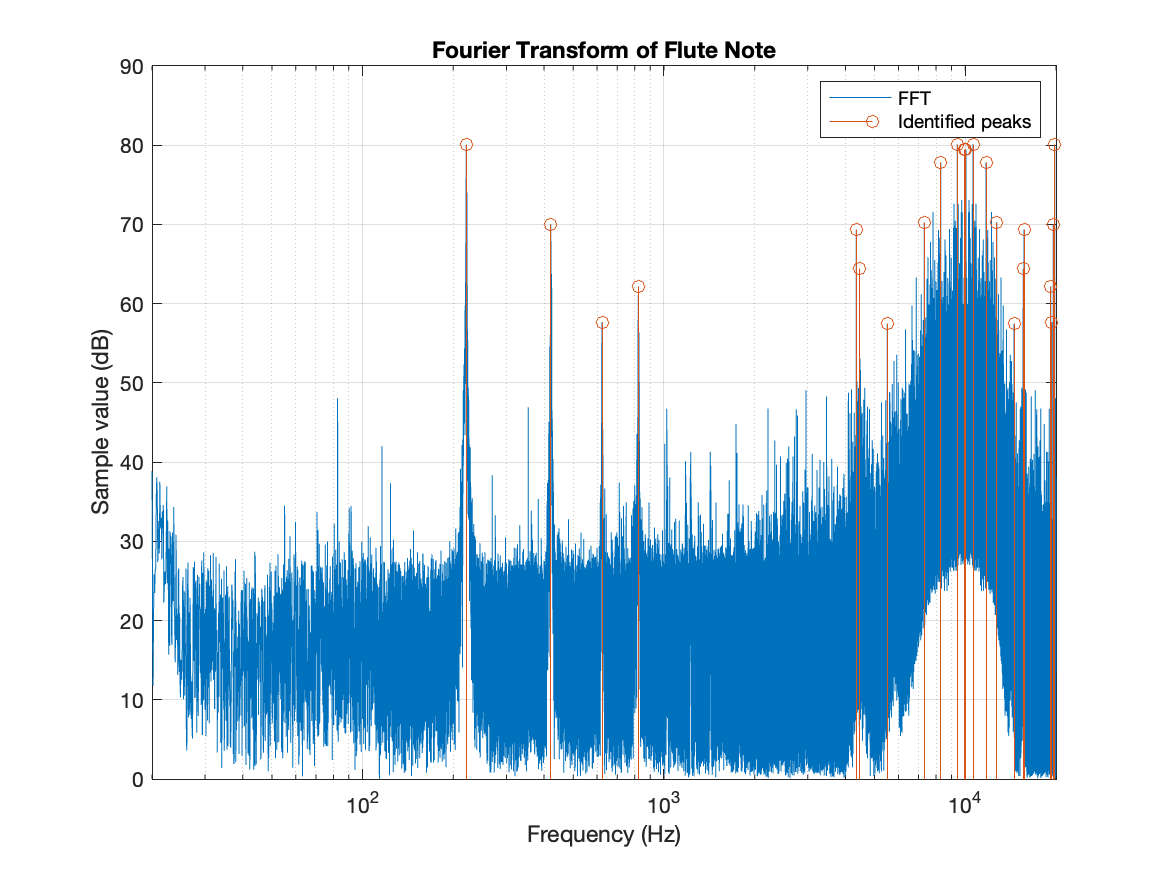
\includegraphics[width=\linewidth]{images/FFTFlute.png}%
                    \centering
                    \caption{Fourier transform of the flute recording.}
                    \label{FFTFlute}
                \end{minipage}
            \end{figure}

            \begin{figure}[H]
                \centering
                \begin{minipage}{.49\textwidth}
                    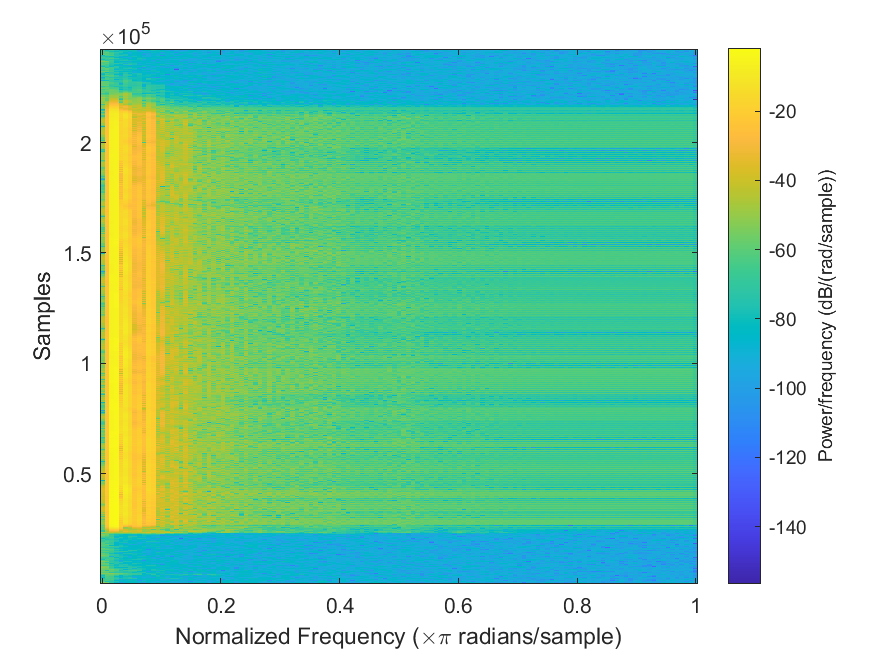
\includegraphics[width=\linewidth]{images/fluteSpec.png}%
                    \centering
                    \caption{Spectrogram of the flute recording.}
                    \label{fluteSpec}
                \end{minipage}
                \begin{minipage}{.49\textwidth}
                    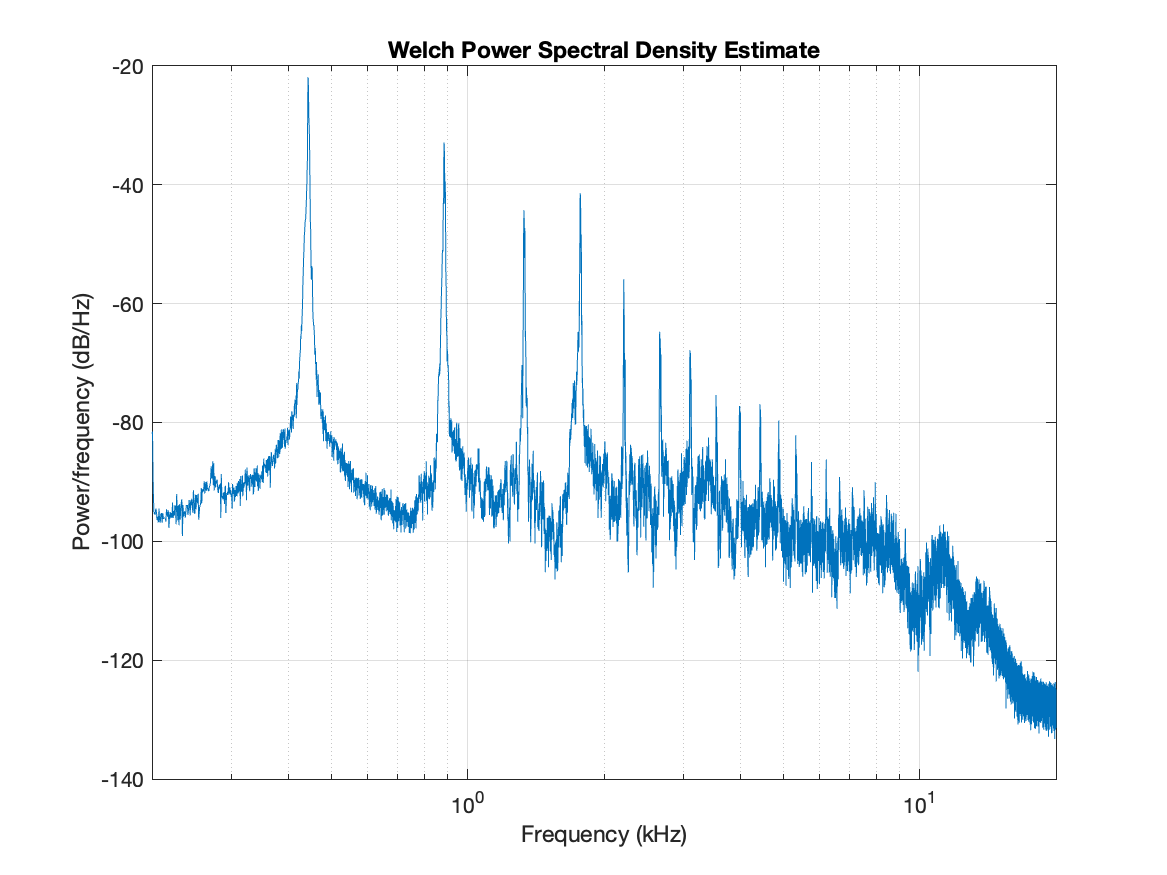
\includegraphics[width=\linewidth]{images/fluteWelch.png}%
                    \centering
                    \caption{Welch-algorithm frequency analysis of the flute recording.}
                    \label{fluteWelch}
                \end{minipage}

            \end{figure}

            From Fig. \ref{timeDomainFlute} it can be observed that the flute has a similar attack, smaller decay and a more constant sustain compared to the mandolin.
            Figures. \ref{fluteWelch} and \ref{FFTFlute} show a harmonically rich frequency content.
            Upon further inspection, the first four harmonics are read as $f_n = 220, 421, 623, 823\text{Hz}$.
            These values roughly correspond to both odd and even harmonics of the fundamental $f=220\text{Hz}$.
            Figure. \ref{fluteSpec} shows that harmonic content, especially in the lower end of the spectrum, remains fairly constant throughout the duration of the note.
            This suggests that FM is a suitable method for synthesis, as the fine control over harmonics given by TVPAS is not particularly important.
            

    \subsection{Synthesis}
        \subsubsection{Additive Synthesis}
            Additive synthesis follows the intuition found in Fourier analysis: Any continuous signal is a sum of an infinite number of sine waves.
            Thus, it should be possible to recreate any given signal by breaking it down into it's frequency components, and reproducing these frequency components as sinusoids weighted according to the frequency domain of the analysed signal.
            A programmatic approach was taken in MATLAB: A fourier transform of the recorded signal would return a set of data that may be parsed to find the frequencies of the dominant harmonics of the Mandolin.
            This was implemented by feeding the result of the fourier transform into MATLAB's \texttt{findpeaks()} function, which allows the user to define arguments as to the minimum height and prominence of maxima within a set of data, these maxima would be the harmonics.
            Using \texttt{findpeaks()} required some trial and error adjusting function arguments to avoid less useful peaks within the Fourier transform.
            The found frequencies and their amplitudes would then be substituted into a looping summation of generic sine wave formulae, to produce the output: a complex signal with a similar frequency response to the input; importantly with the same harmonics.
            This formula is shown in Eq.\ref{sineFormula}.
            \begin{equation}
                y[t] = \sum_{n=1}^{N} A_n \sin{(2 \pi f_n t)}, \text{ where: } n = \text{harmonic number}
                \label{sineFormula}
            \end{equation}
            This produced a signal which contained similar frequency-domain characteristics as the Mandolin recording, but had no amplitude envelope.
            Thus when played using MATLAB's \texttt{sound()} function, the synthesised sound was missing the characteristic plucked attack of a Mandolin.
            To compensate for this, an amplitude envelope was extrapolated from the recorded signal using MATLAB's \texttt{env()} function.
            When passing only the sample value vector to \texttt{env()} a vector of the absolute value of the sample values is returned.
            This is problematic; the sharp changes in amplitude, as shown in Fig. \ref{envMando}, will result in additional high-frequency components being added to the signal when the envelope is applied to the synthesized sound.
            \begin{figure}[H]
                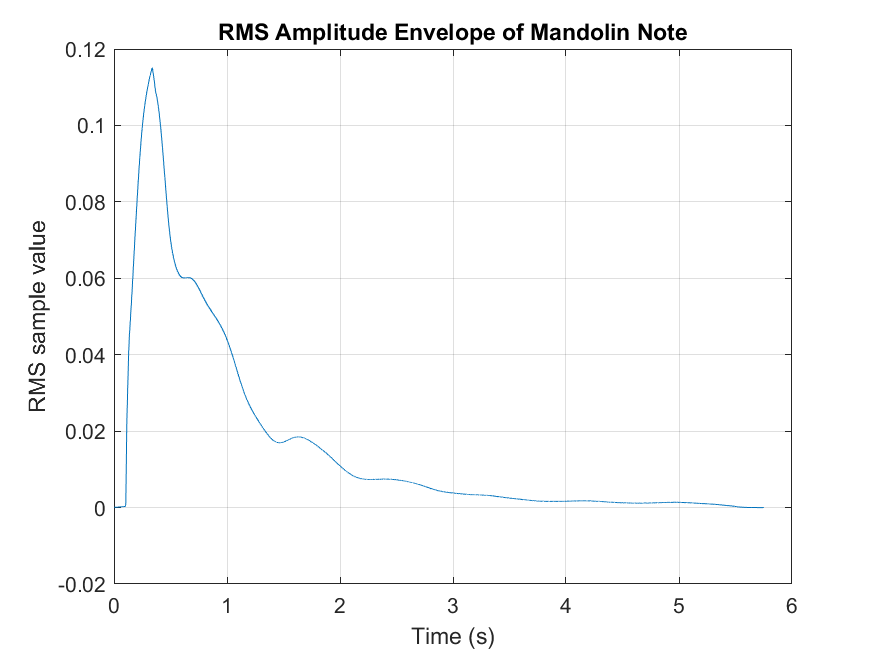
\includegraphics[scale=0.5]{images/envMando.png}%
                \centering
                \caption{Envelope reflecting the absolute value of each sample.}
                \label{envMando}
            \end{figure}
            Passing an \texttt{'rms'} argument to \texttt{env()} gave a smoother envelope than simply taking the absolute value of the time-domain waveform, this addressed the aforementioned problems with using an absolute envelope.
            This new envelope is seen superimposed in Fig. \ref{envMando}.
            To apply the envelope, simply multiplying it with the synthesized signal was sufficient.
            Figure \ref{additiveEnv} shows the envelope applied to the synthesized signal.
            Comparing to Fig. \ref{timeDomainMando}, we can see a similarity in the time-domain.
            \begin{figure}[H]
                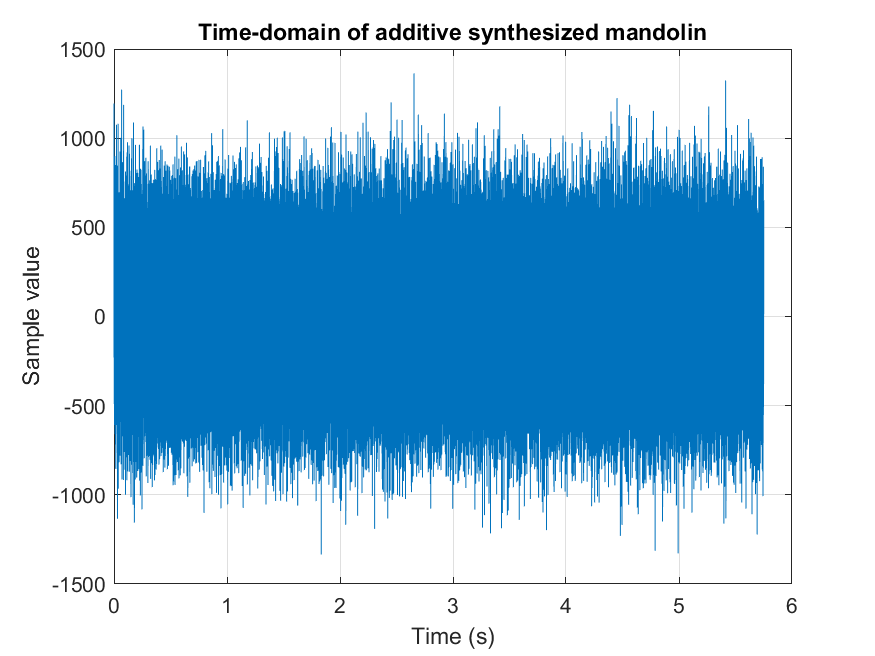
\includegraphics[scale=0.5]{images/additiveEnv.png}%
                \centering
                \caption{Time-domain of the synthesized signal with envelope applied.}
                \label{additiveEnv}
            \end{figure}

            Whilst the spectrograms shown in Figures \ref{specMando1} and \ref{specWaterfallMando1} were useful in illustrating and conveying the amplitude envelopes of a large amount of frequencies across the recording's spectrum, the additive synthesis method chosen chooses to reproduce only a specific few of the harmonic components of the recorded signal.
            Thus, a new spectrogram function will have to be computed targeting the harmonics identified with \texttt{findpeaks()}.
            MATLAB's spectrogram function thankfully allows for an argument to define target frequencies, so after passing the frequency vector extrapolated from \texttt{findpeaks()}, a two-dimensional array of amplitude envelopes for each identified frequency was generated.
            This spectrogram can be seen in Figs.\ref{specMando2} \& \ref{specWaterfallMando2}.
            \begin{figure}[H]
                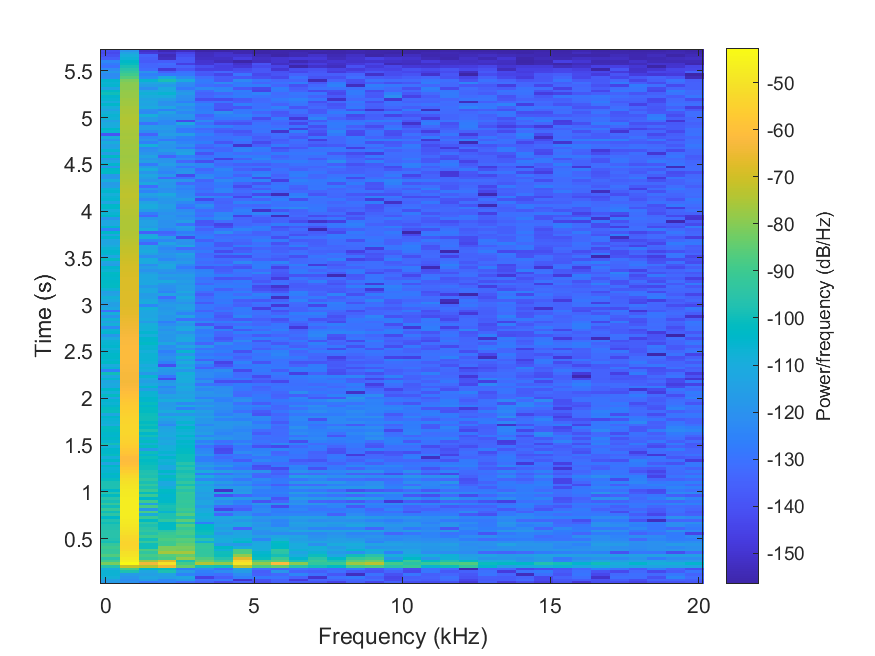
\includegraphics[scale=0.5]{images/specMando2.png}%
                \centering
                \caption{Mandolin sample value over time.}
                \label{specMando2}
            \end{figure}
            \begin{figure}[H]
                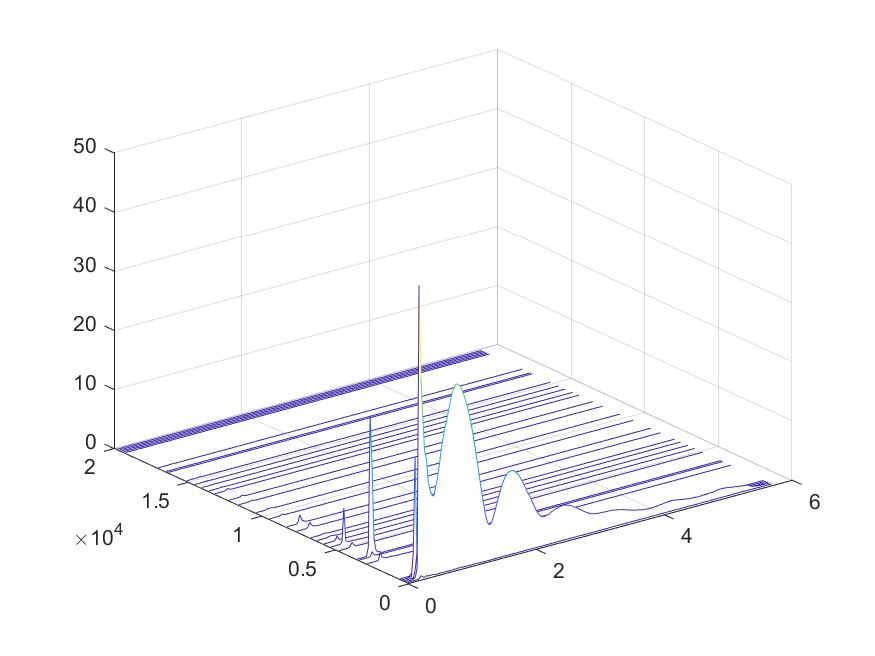
\includegraphics[scale=0.5]{images/specWaterfallMando2.png}%
                \centering
                \caption{Mandolin sample value over time.}
                \label{specWaterfallMando2}
            \end{figure}

        \subsubsection{Frequency Modulation Synthesis}
            To emulate the recorded flute, frequency modulation (FM) synthesis was used.
            FM synthesis generates signals with rich harmonic content using only two waveforms, as opposed to the theoretically limitless number of oscillators typically used in additive synthesis.
            Instead of summing the oscillators as in additive synthesis, the two oscillators are multiplied.
            The two waves are referred to as the ``carrier'' and the ``modulator''
            Chowning elaborates on the relationship between the two waves: ``In FM the instantaneous frequency of a carrier wave is varied according to a modulating wave, or modulating frequency''~\cite{chowning1973synthesis}.
            This is reflected in the general equation for FM synthesis:
            \begin{equation}
                \begin{split}
                    y(t) &= A\sin{(\omega_c t + I\sin{\omega_m})} \\
                    \text{Where:} \\
                    A &= \text{Amplitude coefficient} \\
                    \omega_c &= \text{angular frequency of carrier} \\
                    \omega_m &= \text{angular frequency of modulator} \\
                    I &= \text{modulation index}
                \end{split}
            \end{equation}
            \\
            Returning to Chowning's paper, parameter sets and methods for use of the above equation targeting the sound of certain instruments are given.
            Chowning states that a woodwind sound may be achieved: ``By setting the carrier frequency to be an integral multiple of the modulating frequency, or by making the index function inversely proportional to the amplitude function''.
            To implement this, a frequency equivalent to the identified fundamental tone of the flute, $f_c=220\text{Hz}$ was used for the carrier. 
            The modulator was then set to a value of $f_m = f_c * 4 = 880\text{Hz}$.
            By making the index function $I = \frac{\delta_f}{f_m}$ both of Chowning's listed woodwind criteria are met.
            A fourier transform of the output of the frequency modulation synthesis is shown in Figs.\ref{synthFluteFFT} \& \ref{synthFluteSpec}.
            
            \begin{figure}[H]
                \centering
                \begin{minipage}{.49\textwidth}
                    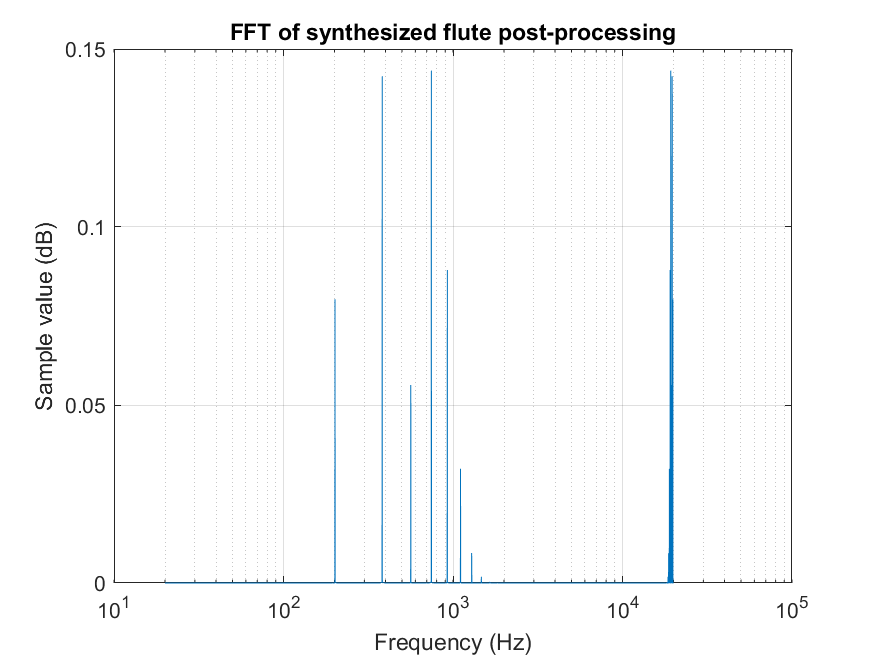
\includegraphics[width=\linewidth]{images/synthFluteFFT.png}%
                    \centering
                    \caption{FFT of output of FM synthesis.}
                    \label{synthFluteFFT}
                \end{minipage}
                \begin{minipage}{.49\textwidth}
                    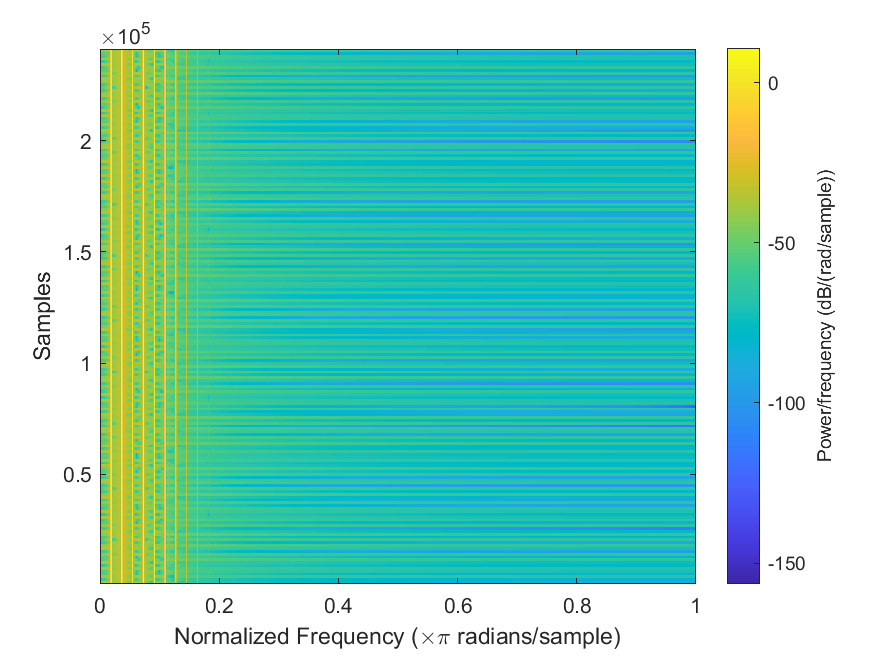
\includegraphics[width=\linewidth]{images/synthFluteSpec.png}%
                    \centering
                    \caption{Spectrogram of output of FM synthesis.}
                    \label{synthFluteSpec}
                \end{minipage}
            \end{figure}
            The spectrogram in Fig. \ref{synthFluteSpec} shows a good similarity to the frequency response over time shown in Fig. \ref{fluteSpec}.
            Thus, the next step was to match the amplitude response of the synthesized note to the recorded note.
            A programmatic amplitude envelope using the exact same \texttt{env()} function as the mandolin synthesis was generated.
            Also, a manual attack-decay-sustain-release envelope was drawn in MATLAB from observation of Fig. \ref{timeDomainFlute} and used to weight the amplitude of the signal over time.
            The manual and programmatic amplitude envelopes are shown in Figs.\ref{ADSR} \& \ref{envFlute}.
            \newpage
            \begin{figure}[H]
                \begin{minipage}{.49\textwidth}
                    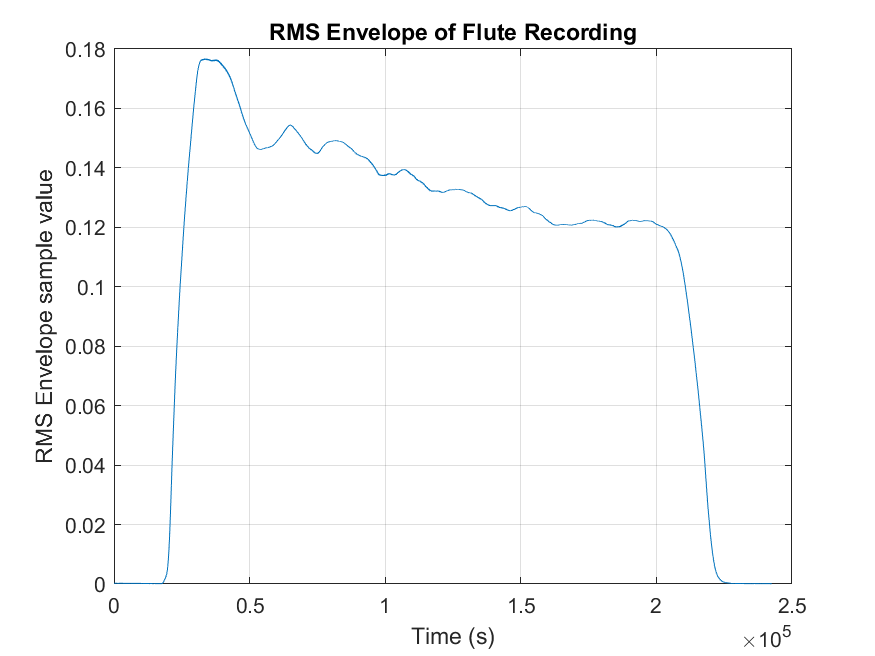
\includegraphics[width=\linewidth]{images/envFlute.png}%
                    \centering
                    \caption{RMS amplitude envelope of recorded flute.}
                    \label{envFlute}
                \end{minipage}
                \begin{minipage}{.49\textwidth}
                    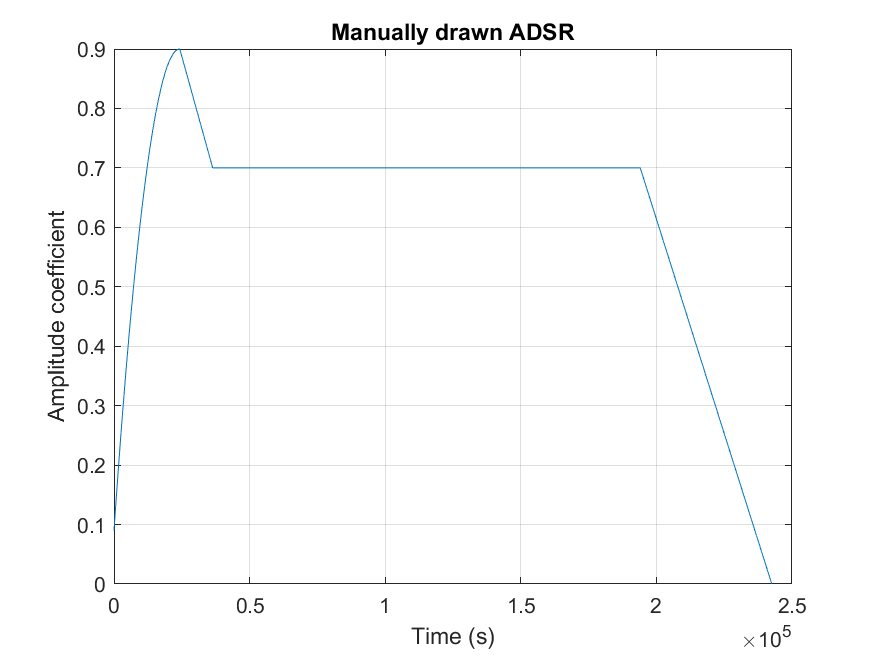
\includegraphics[width=\linewidth]{images/ADSR.png}%
                    \centering
                    \caption{Manually drawn ADSR.}
                    \label{ADSR}
            \end{minipage}
            \end{figure}
            Listening back to the synthesized note with the manual and programmatic amplitude envelopes applied revealed the manual envelope to sound ``unhuman'' with none of the minor fluctuations in amplitude caused by an air-reed and slightly inconsistent airflow from the mouth.
            Whilst this may be fixed by adding low-frequency amplitude modulation to achieve a subtle ``tremelo'' effect, the programmatic amplitude envelope was chosen instead to keep things simple.
            
            Looking back to Fig. \ref{synthFluteFFT} a large amount of clustered high frequency content can be seen and is also audible on playback of the synthesized sound; this is unlike the flute recording.
            To combat this, a 16\textsuperscript{th} order low-pass Butterworth filter was generated using \texttt{butter} and applied to the synthesized signal using \texttt{filter()}.
            In addition, a low-amplitude noise signal was summed with the synthesized tone to attempt to recreate the ``airy'' or ``breathy'' nature of the flute's sound.
            A plot of the FM synthesis after going through this processing is seen in Figs.\ref{synthFlutePostProcessFFT} \& \ref{synthFlutePostProcess}
            \begin{figure}[H]
                \centering
                \begin{minipage}{.49\textwidth}
                    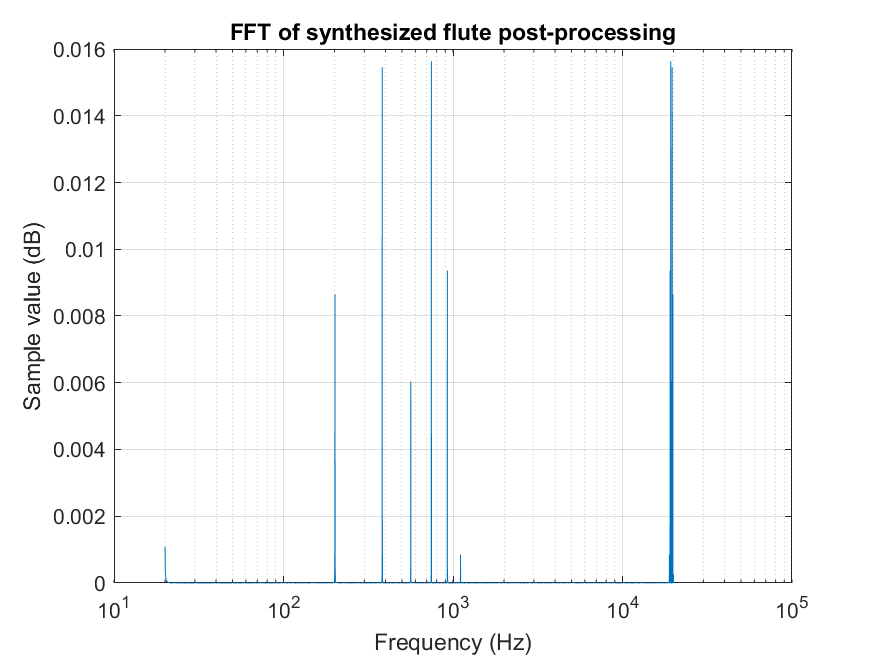
\includegraphics[width=\linewidth]{images/synthFlutePostProcessFFT.png}%
                    \centering
                    \caption{FFT of post-processing FM synthesis.}
                    \label{synthFlutePostProcessFFT}
                \end{minipage}
                \begin{minipage}{.49\textwidth}
                    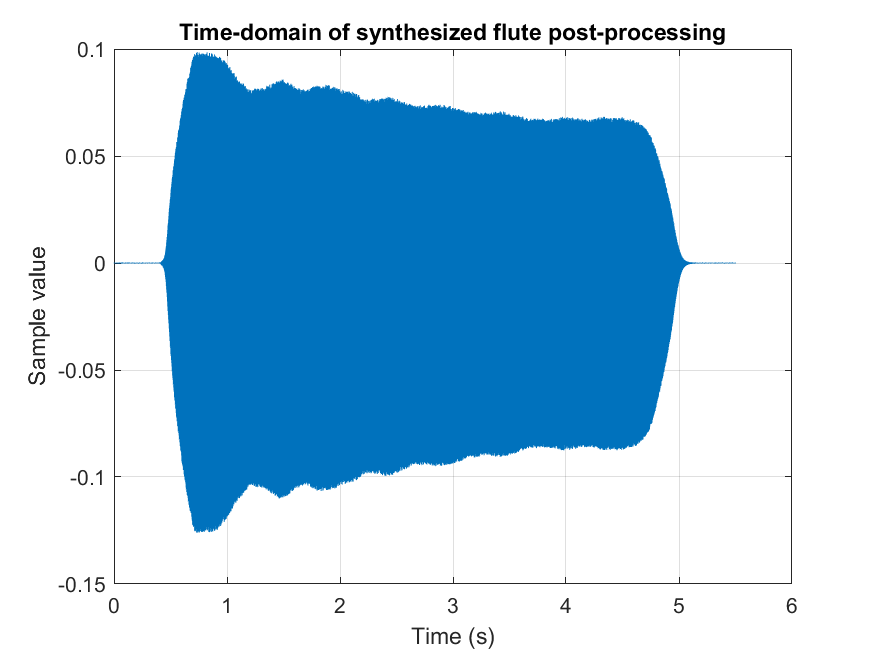
\includegraphics[width=\linewidth]{images/synthFlutePostProcess.png}%
                    \centering
                    \caption{Time-domain of post-processing FM synthesis.}
                    \label{synthFlutePostProcess}
                \end{minipage}
            \end{figure}

\section{Discussion and Conclusions}
\section{Appendix}
\subsection{Code}



\bibliographystyle{IEEEtran}
\bibliography{theBib.bib}

\end{document}


